\section {System Overview\\}

\subsection{Design Goals and Rationales\\}
The design of the PushUp server is driven by the following rationales.
\begin{itemize}
\item {\bf Large Concurrent Connections}:
    As the long polling technologies requires the server to keep the polling
    request active for a period of time, large number of concurrent clients 
    will generate lots of active connections. One of the most goal of PushUp
    is to minimize the cost of maintaining these active concurrent connections,
    which can in turn enhance the system's scalability.
     
    The key to reduce the cost is the event-driven concurrency architecture.
    Unlike the multiprocessing or multithreading models, the event-driven model 
    requires much less resource to maintain the connections, avoids context
    switches between threads and expensive lock operations.

\item {\bf Generality}: 
    Although event-driven concurrency significantly 
    reduce the maintenance cost, it is impractical to have all the web 
    server to be implemented in event-driven programming style. Thus, it makes
    sense to offer a dedicated long polling services, which enables all the web
    servers to obtain the long polling functionality with minimal effort.

    Moreover a general long polling service provider prevents web servers from 
    re-inventing the wheels and, according the Linus Law\cite{Linus} "
    Many eyes make bugs shallow", helps to make the service more robust.
 
\item {\bf Low Latency}: Adding an intermediate layer in between of the 
    clients and web servers will inevitably create some overhead. 
    The PushUp server should make sure that the extra costs be controlled within
    an ``acceptable" range. In the evaluation section we will carefully examine
    the latency of the PushUp servers.

\item {\bf Scalability}: The PushUp Server is designed to handle large number
    of active connections. In later sections we well further explore 
    mechanisms that help the PushUp scales better.  

\end{itemize}

\subsection{System Architecture\\}

Figure \ref{fig:architecture} shows the overall architecture of the PushUp servers.
The PushUp server is essentially a specialized message queue, with clients 
acting as the subscribers and the web server the publishers.

When a client initites an http request, the reverse proxy acts as the web front end,
which will:
\begin{itemize}
    \item[1] Forwards the normal(non-polling) http requests to the corresponding 
             web servers.
    \item[2] Intercepts the polling http requests and sends a subscription request to 
             the PushUp servers.
\end{itemize}

The reverse proxy is a kind of proxy that retrieves
resources on behalf of a client from one or more 
servers.\cite{ReverseProxy}. In this case, the reverse
proxies hide the existence of the origin servers (the 
web servers and PushUp servers) and presents the clients
a uniform interface.

On the other end, the web servers can send the publication requests to the 
PushUp servers in order to inform interestd clients with the latest updates.

As suggested figure \ref{fig:architecture}, there can be more than one PushUp 
servers working together. Both subscription and publication will go through a 
load balancer, which distributes these requests to one of the servers. All 
PushUp servers are ``identical" to each other. That is, a subscriber can 
subscribe to any of PushUp servers and the publisher can 
publish message to whatever PushUp server. We will discuss more details in next
section.

\begin{figure}[htb!]
\centering%
    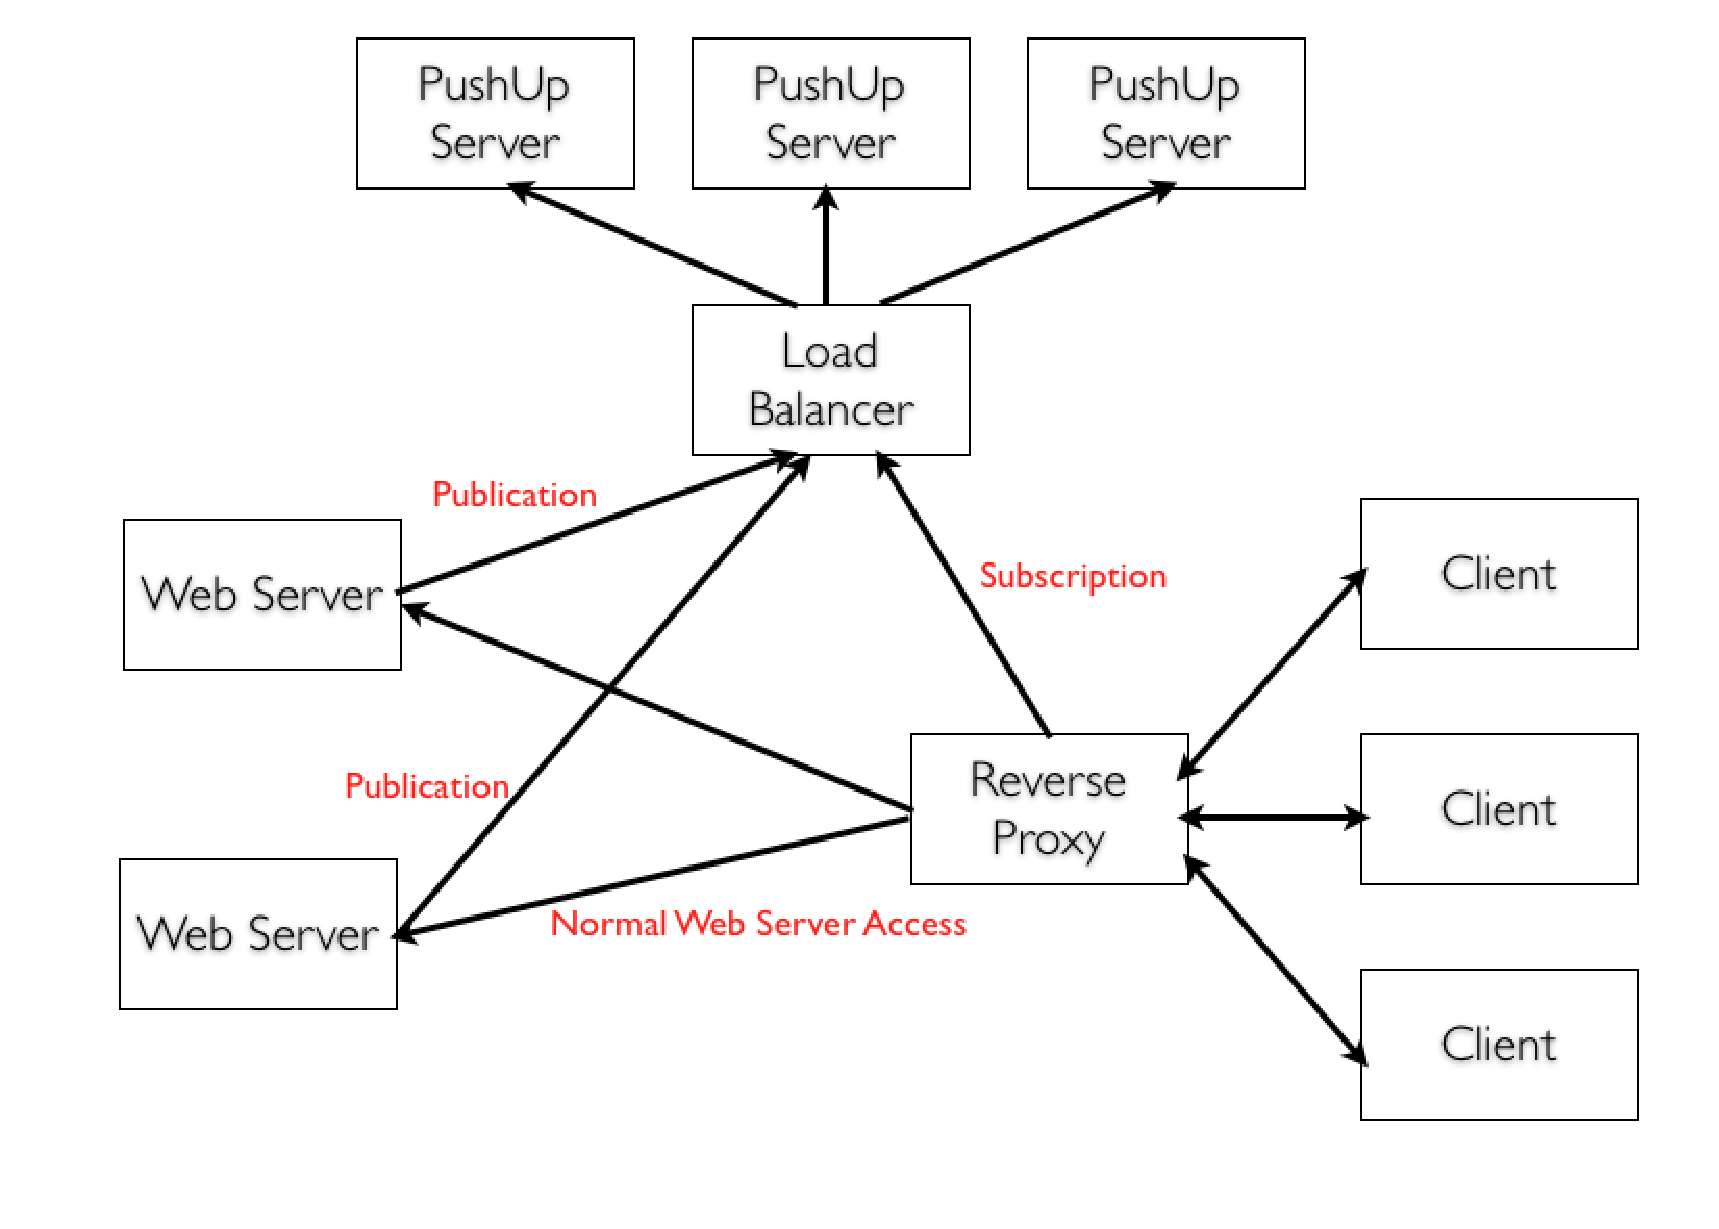
\includegraphics[scale=0.30]{figures/pushup.eps}
    \caption{PushUp Architecture}
    \label{fig:architecture}
\end{figure}

